\documentclass[11pt, a4paper]{article}
\usepackage{graphicx}
\usepackage{amsmath, bm}
\usepackage{natbib}
\usepackage[utf8]{inputenc}    
\usepackage{natbib}
\usepackage[usenames,dvipsnames]{xcolor}
\usepackage[left=2cm,right=2cm,top=2cm,bottom=2cm]{geometry}
\usepackage{hyperref}
\usepackage[outdir=./]{epstopdf}
\usepackage{lscape}
\usepackage{multirow}
\usepackage{booktabs} % Create TABS
\usepackage{array,arydshln}  % CREATE DASH LINE
\title{Identification of stably expressed genes in RNA-Seq data of  Arabidopsis}
\date{} % Today's date or a custom date

\begin{document}
\maketitle


\section{Introduction}

\textbf{Why is normalization important}
RNA sequencing (RNA-Seq) has become the technology of choice for transcriptome profiling, and has gained popularity over the last few years. A key task of RNA-Seq analysis is to detect differentially expressed (DE) genes under various experimental or environmental conditions. Although the ability of DE detection between samples is associated with transcript length\citep{oshlack2009transcript}, \cite{bullard2010evaluation} demonstrated that the choice of normalization has the greatest impact. Previous study showed that \textit{between-sample} effects, e.g., sequencing depths, flow-cell/library preparation effects (\cite{bullard2010evaluation}, \cite{robinson2010scaling}), as well as \textit{gene-specific} effects, e.g.,  gene length or GC-contents (\cite{risso2011gc}, \cite{hansen2012removing}) are nuisance effects that may have implications on normalization, and therefore on inference of expression level and subsequent (Gene Ontology) analysis.  \\

\textbf{Why is stably expressed gene important}
Studying stably expresed genes are important Stably expressed genes are used as reference genes for normalization. During the past few years, a number of normalizaiton procedures have been proposed to address different types of unwanted nuisance effects (see \cite{dillies2013comprehensive}, \cite{risso2014nat} for a comprehensive review).\cite{bullard2010evaluation} evaluated a global normalization method: counts for a "housekeeping" gene expected to be stably expressed under different biological conditions. \cite{risso2014nat}  proposed RUVg approach that uses negative control genes, whose expression levels are assumed to be unaffected by covariates of interest. 
 Besides, in expression study, a high correlation between translational signiture and mRNA level is found in human stably expressed genes\citep{line2013translational}. In that paper, an significant increase in mRNA variation prediction was obtained by selecting genes that are stably expressed in more than 1 tissue.\\
%One such example of stably expressed genes are so-called "housekeeping genes", which are involved in basic cell maintenance and, therefore, are expected to maintain constant expression levels in all cells and conditions. 

\textbf{Stably expressed genes are subject to change}
Traditionally, in microarray study so-called "housekeeping genes"(HKGs) are used as sreference genes for normalization. HKGs are typically constitutive genes that maintain basic cellular function, and therefore are expressed at relatively constant levels in non-pathological situations. However, such HKGs are found to be subject to change, either under varying experimental protocols, or different organs of a given species. For example, in the microarray analysis of classical model plant \textit{Arabidopsis thaliana} (Arabidopsis), \cite{czechowski2005genome} showed that traditional HKGs such as ACT2, TUB6, EF-1$\alpha$ are not necessarily good candidates for normalization.  Instead, they suggested 10 new sets of reference genes in terms of expression stability,  by investigating 721 arrays of 323 conditions throughout development. Interestingly, \cite{dekkers2012identification} identified another set of stable genes specifically for Arabidopsis seed from an analysis of 16 samples, which shared about only 3\% reference genes with top 100 in \cite{czechowski2005genome}.  \cite{hruz2011refgenes} pointed out that universally stably expressed genes may not exist and that a subset of stably expressed genes from a specific biological context has less variability than those identified across varying tissues and conditions.\\

\textbf{Ready to move to next section}
Although stably expressed genes by the two studies don't share much in common, \cite{czechowski2005genome} and \cite{dekkers2012identification} adopted  similar approach for statistical analysis, and both used Arabidopsis microarray data. Briefly, for each gene the mean expression and the standard deviation (SD) over all biological samples are calculated, and the coefficients of variation (CV), which is the ratio of SD and mean expression, are obtained. Genes with lower CVs are expected to be more stably expressed. This simple approach, however, does not provide us any information about possible sources, except the amounts,  of variation.\\ 

\textbf{What is our goal and the approach}
Our question of interest is whether stably expressed genes are consistent between RNA-Seq and microarray technologies. Over the last few years,  the exponential growth in RNA-Seq study provides a large amount of Arabidopsis data and enables us to address the question mentioned above. The aim of this study is two fold: 1) to quantify the source of variation of gene expression level, and 2) to identify a list of stably expressed genes potentially for addressing normalization issues. RNA-Seq data are presented in the form of read count matrix, each row representing one gene and each column representing one sample. With covariates (e.g. lab, treatment) taken into account,  the classical regression models may not be appropriate. In this paper, we apply a generalized linear mixed model (GLMM)\citep{mccullagh1989generalized} to explore stably expressed genes. For each gene,  we assume a common mean for the read count across samples, with an offset term accounting for library sizes adjustment. We also define three random terms to capture \textit{between-sample}, \textit{between-treatment} and \textit{between-experiment} variation. \\ 
 
 \textbf{what are the results}
Analyses of 165 biological samples from 18 different Arabidopsis experiments show that sets of stably expressed genes are, to some extent, consistent between RNA-Seq studies and microarray studies. In addition, by partitioning total variation of expression level into between experiment, between treatment and between biological sample variations, we found the major source of variability comes from experiment, followed by treatment, whereas sample variability contributes the least to total variation.  Our study shows that normalization factors calculated via  \cite{anders2010differential} using the list of stable genes are robust against different data sets. 

\section{Data}

\textbf{Source of Data} SRA format files of Arabidopsis were retrieved from NCBI  (\url{http://www.ncbi.nlm.nih.gov/}), and then converted to \verb"FASTQ" using \verb"SRA Toolkit(version 2.3.5-2)". The reference genome of Arabidopsis is obtained  through the Ensembl plants FTP server (\url{http://plants.ensembl.org/info/data/ftp/index. html}). As suggested by \cite{anders2013count},  "FASTA(DNA)" link rather than "FASTA(cDNA)" is selected because samples are aligned to the genome, not the transcriptome. Alignments were done by  \verb"align()" and read counts were summarized by \verb"featureCounts()". Both functions are in R package \verb"Rsubread (version 1.14.2)"  \citep{shi2013subread},\nocite{liao2013subread} using default option except that the reference genome is set to be \verb"Arabidopsis_thaliana.TAIR10.22.gtf". All procedures were implemented by R in an automatic manner and code is available upon request.  We obtained 165 biological Arabidopsis samples from 18 experiments, which are named by their corresponding GEO accession number in NCBI.  A brief description of each experiment can be found in supplementary material, or in NCBI website via the unique accesion number provided.\\

\textbf{Details of Data} As demonstrated in previous works (\cite{czechowski2005genome}, \cite{hruz2011refgenes}, \cite{dekkers2012identification}), transcriptomes vary across different tissue types or development stages. We therefore grouped the samples into three Arabidopsis data sets in the following manner: \textbf{Set 1} consists of 72 biological samples that come from 9 experiments of Arabidopsis seedling under 29 treatments with different experimental/environmental conditions or genotypes. The ages of seedlings range from 2 to 10 days. \textbf{Set 2} has a sample size of 39 that consists of 5 experiments with 16 treatments. Each experiment corresponds to one specific tissue types, that is, flower, leaf, seed, carpel and hypocolty. \textbf{Set 3} consists of 5 experiments conducted specifically for leaf, with a total number of 60 biological samples from 28 different treatments. Note that  Set 2 and Set 3 overlap with each other by experiment GSE48235.  \\

\textbf{Pre-processing of data} The library layout for all samples was single end, and pair end data were not included. The data sets from different experiemnts of arabidopsis were then merged by gene IDs.  Furthermore, non-informative rows, such as features that are not of interest or those having low overall counts were removed, as suggested by\cite{anders2013count}. We adopted this suggestion in our data analysis, not only because rows with small read counts provides little information about expression level,  but also that such rows will cause convergence failure in the regression models. All three data sets  were filtered by the criteria "averagely, 3 counts per gene per sample" to avoid computational issues. We obtained 22334 genes for set 1,25239 genes for set 2, and 21290 genes in set 3, out of the original 33,602 genes. 
%We searched all the arabidopsis data available at NCBI (up to August 31, 2014) and processed some of the SRA format data to obtain RNA-Seq read count table. However, due to various reasons (platform, sequencing depth??), data quality are not consistent. Therefore, after a normalization procedure using "AH2010" method implemented in NBPSeq\nocite{di2014package},  we chose data sets with normalization factor ranging from 0.75-1.25 (subject to change). 

\section{Methods}
Considering the fact that the response is in the form of count, we implemented the analysis under generalized linear mixed model framework\nocite{mccullagh1989generalized}. Given the randomness of experimental data we collected, the experiments, as well as the treatments each experiment received, are considered to have random effects. Also because treatments are nested in experiments, they are treated as nested effects under experiments. We further specify another random effect term accounting for variation among biological samples.  The statistical analysis is implemented using Poisson regression with random effects.

Let $Y_{ijkl}$ denote the read count for $i$th gene in $j$th observational unit of $k$th treatment group in $l$th experiment ( {\color{red} this notation agrees with the NBP paper, except that I added $l$ here to denote experiment}), and index $i$ is suppressed herein since only one gene is evaluated at a time by our model. It is assumed that this read count to follow a Poisson distribution, i.e.  
% {\color{blue} Probably we should say for a particular gene, Let $Y_{ijk}$ denote the read count for $i$th sample in $j$th treatment of $k$th experiment.}
% In this section, instead of assuming $Y_{ij}$ to be negative binomial random variable, we here impose a Poisson distribution with random term adjusting for  extra variation. Specifically, for a particular gene $i$ (index suppressed here)
  \[Y_{jkl}\sim \text{Poisson}(\mu_{jkl})\]
  We further allow the mean $\mu_{jkl}$ to vary across samples and experimental conditions (treatments, organs, etc.) by imposing the following model 
  \begin{equation}\label{q1}
   \log( \mu_{jkl}) = \xi + \log(R_{jkl}N_{jkl})+ \alpha_l + \beta_{k(l)} + \epsilon_{jkl} 
  \end{equation}
 %   \[ \log( \mu_{ijk}) = \xi + \log(R_{ijk}N_{ijk})+ \alpha_k + \beta_{j(k)} + \epsilon_{ijk} \]
  \[\alpha_l\sim N(0, \sigma^2_1),\] 
  \[\beta_{k(l)}\sim N(0, \sigma^2_2),\]
   \[\epsilon_{jkl}\sim N(0, \sigma_0^2)\]
  where $\alpha$  is the random effect for experiments,  $\beta$ is treatment effect nested in experiments, and $\epsilon$ is the random effects for biological samples. It is also assumed that $\alpha, \beta$ and $\epsilon$ are mutually independent. The term $\log(R_{jkl}N_{jkl})$ serves as an offset accounting for library size adjustment, and $N_{jkl}, R_{jkl}$ are obtained by DESeq normalization \citep{anders2010differential}. Briefly, a pseudo-reference sample is created by taking the geometric mean across samples for each gene. Then the normalization factor for sample $j$ is estimated as the median of the fold-changes between sample $j$ and reference sample over all genes. \\
  
  The density function of $\bm Y=(Y_1, \ldots, Y_n)'$ given $\bm \mu= (\mu_1, \ldots, \mu_n)'$ is 
  \[f(\bm Y|\bm \mu )=\prod_{ j, k,l}f(y_{jkl}|\mu_{jkl})=\prod_{j,k,l}\frac{[\mu_{jkl}]^{y_{jkl}}\exp(-\mu_{jkl})}{y_{jkl}!}\]
A re-expression of  (\ref{q1}) in matrix form gives 
\[\log\bm \mu=\log{\bm{NR}} + \bm \xi + \bm {Z_1\alpha} + \bm{Z_2\beta} + \bm \epsilon \]
where $\bm \xi = \bm 1\cdot\xi$ and $\bm 1$ is a vector of 1s, $\bm Z_1$ is the design matrix for random effect $\bm \alpha=(\alpha_l)$, and $\bm Z_2$ is the design matrix for random effect $\bm \beta $. 
Therefore  $\bm\mu  \sim \log N(\bm \mu_0, \bm \Sigma)$ where 
$$\bm \mu_0 =\bm\xi + \log(\bm {NR})+ \bm {Z_1\alpha} + \bm{Z_2\beta} + \bm \epsilon,$$ 
$$\bm \Sigma = \sigma_1^2\bm {Z_1Z_1'} + \sigma_2^2\bm {Z_2 Z_2'} +\sigma_0^2 \bm I$$
 and $\bm I$ is of dimension $Q$ where $Q$ is the total number of biological samples. 
 And 
 \[f(\bm \mu |\bm \mu_0, \bm \Sigma)=\prod_{j,k,l} \mu_{jkl}^{-1}\cdot \frac{1}{ \sqrt{(2\pi)^Q|\bm\Sigma|}}\exp[-\frac{1}{2} {(\log\bm \mu - \bm \mu_0)^T\bm \Sigma^{-1}(\log\bm \mu - \bm \mu_0)}]\]
 the joint density is then
  \[f(\bm Y, \bm \mu |\bm \mu_0, \bm \Sigma) =\frac{1}{\sqrt{(2\pi)^Q|\bm \Sigma|}}\exp[-\bm 1^T\bm \mu - -\frac{1}{2} {(\log\bm \mu - \bm \mu_0)^T\bm \Sigma^{-1}(\log\bm \mu - \bm \mu_0)}]\prod_{jkl}\frac{[\mu_{jkl}]^{y_{jkl}-1}}{y_{jkl}!}\]
   Therefore the likelihood function or the marginal distribution is 
   \begin{equation}\label{q2}
   L(\xi, \sigma_1^2, \sigma_2^2, \sigma_3^2|\bm Y)=f(\bm Y|\bm \xi, \bm \Sigma)= \int_{\bm{\alpha,\beta,\epsilon}} f(\bm Y, \bm \mu |\bm \mu_0, \bm \Sigma)d\bm \alpha d \bm\beta d\bm \epsilon 
   \end{equation}
where the integrand of (\ref{q2}) can be approximated by Laplace transformation or Gaussian-Hermite quadrature\citep{mcculloch2001generalized}. The estimate of $\bm\theta = (\xi, \sigma_0^2, \sigma_1^2, \sigma_2^2)'$ is obtained by maximizing the log-likelihood. This procedure is implemented by \verb"glmer()"  under package \verb"lme4" (version 1.1.7)  with option  \verb"optimizer= 'bobyqa' " \citep{bates2012lme4}.
 
 Model (\ref{q1}) allows us to specify the design structure in each data set. We assume that genes are mutually independent. We then fit (\ref{q1}) to each gene, through which the variance components are estimated.  The total variation is quantified by $\sigma^2 = \sigma^2_0 + \sigma_1^2 + \sigma_2^2$. The genes are then ranked by their magnitude of total variation in an ascending order. Top ranked genes are considered to be most stable in terms of expression level. 
  
 \section{Results}

  \subsection{Source of variation}
 We estimated all 3 variance components for each gene. As shown in Figure 1, experimental level variance contributes most to the total variation.  The second largest variation comes from treatment level, whereas biological sample has the least amount of variation.  The plots also reveal that data are more homogenous within a specific tissue or organ (subplot A and C, Figure 1) than across different tissue types (subplot B, Figure 1) since the variation is larger in panel B.  
 \begin{figure}[h!]
\begin{center}\label{Fig1}
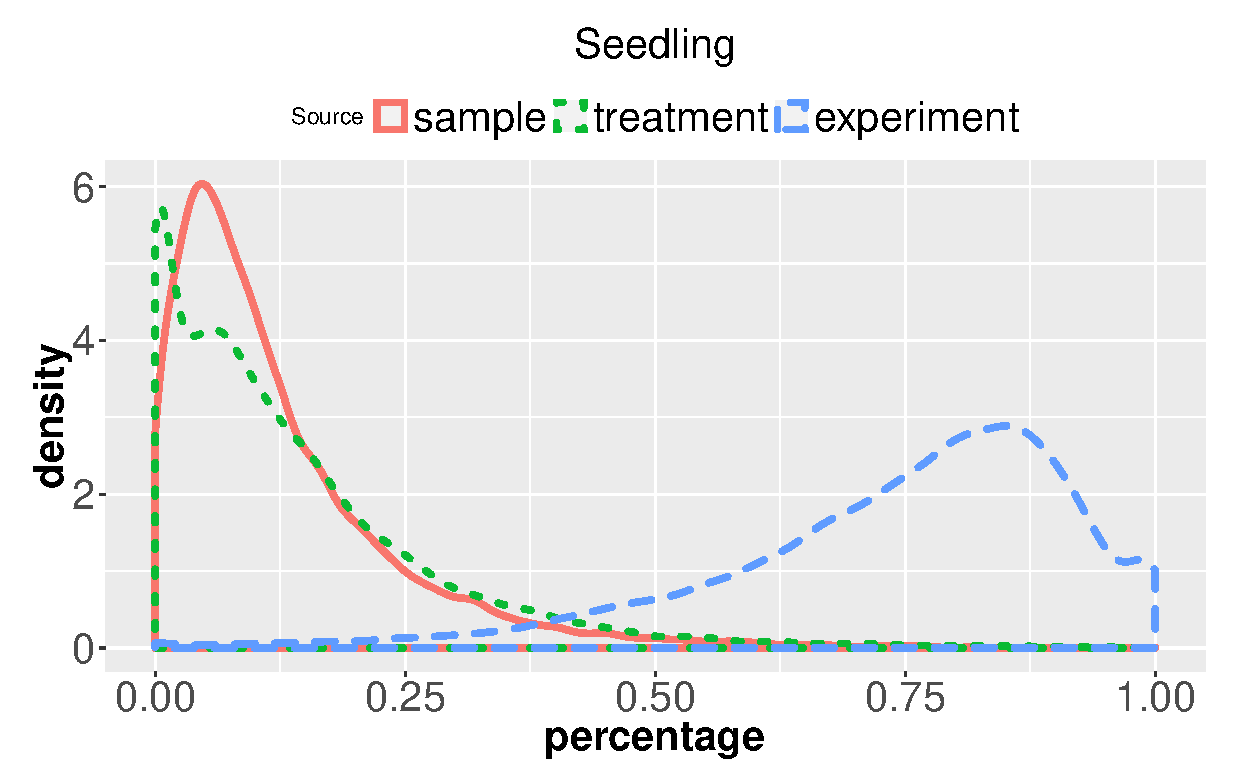
\includegraphics[scale=0.3]{../Figures/var_dens1.eps}
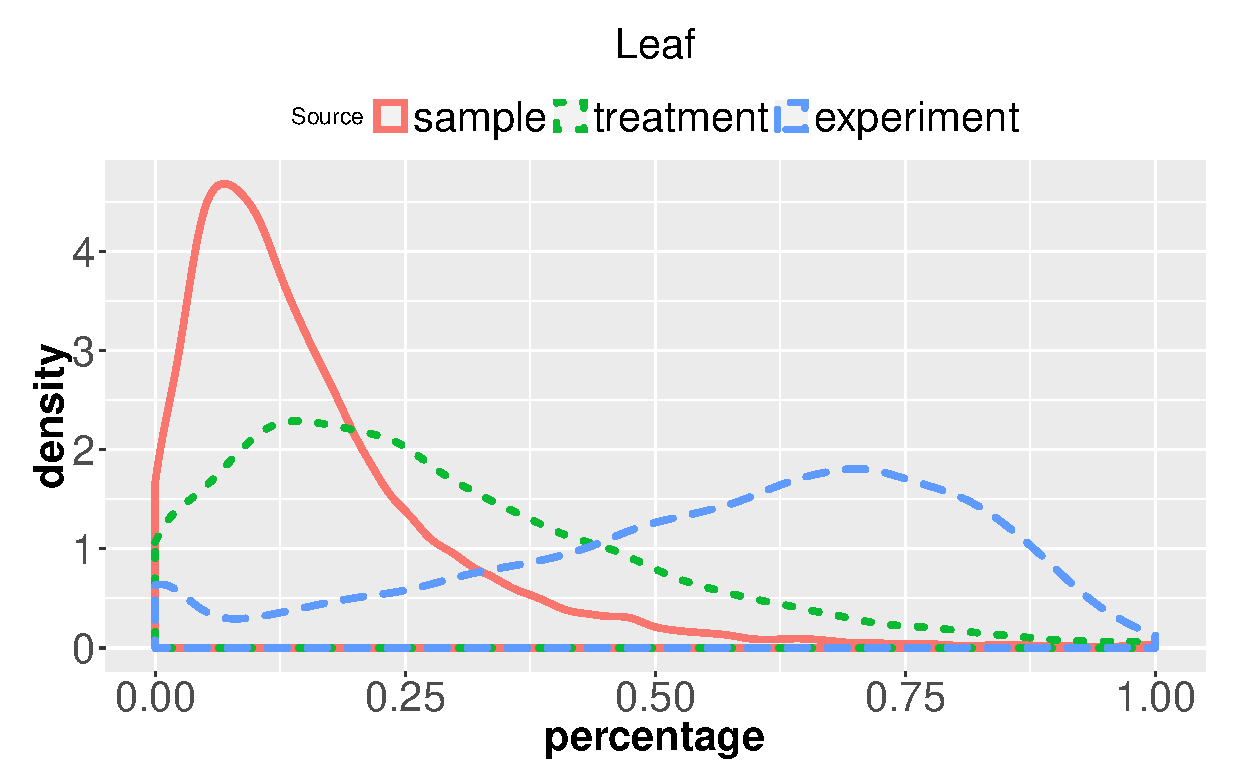
\includegraphics[scale=0.3]{../Figures/var_dens2.eps}
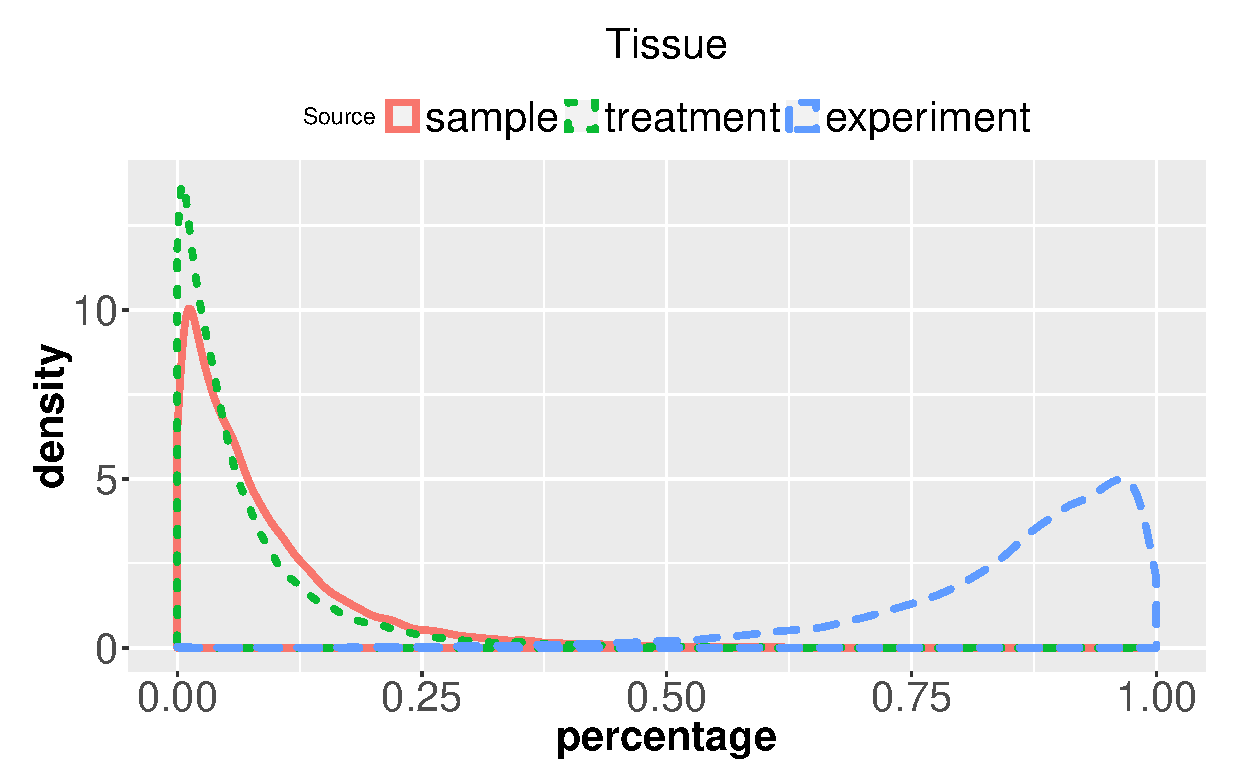
\includegraphics[scale=0.3]{../Figures/var_dens3.eps}
\caption{\label{tag:scaled_diss} source of variation}
\end{center}
\end{figure} 


 \begin{figure}[h!]
\begin{center}\label{Fig1}
\includegraphics[scale=0.3]{../Figures/v1.png}
\includegraphics[scale=0.3]{../Figures/v2.png}
\includegraphics[scale=0.3]{../Figures/v3.png}
\caption{\label{tag:scaled_diss} source of variation}
\end{center}
\end{figure} 

  \subsection{Stably Expressed Genes}
 We listed top 100 genes that are identified as most stably expressed (see supplementary material). Figure 2 shows the normalized CPM (counts per million, $=Y_{ij}/N_j\cdot 10^6$obtained by dividing each column of the count table by the corresponding library sizes and then multiplying $10^6$)\citep{anders2013count} of top 5 stably expressed genes for Set 1, Set 2, and Set 3. As a comparison, we also present five traditional reference genes and five novel stably expressed genes claimed in \cite{czechowski2005genome} (Figure 1). In general, traditional reference genes are not necessarily stable ones.  Novel reference genes are relatively more reliable,  however our analysis shows that not all of them are in top list of stable genes. 

\begin{landscape}
 \begin{figure}[H]
\begin{center}
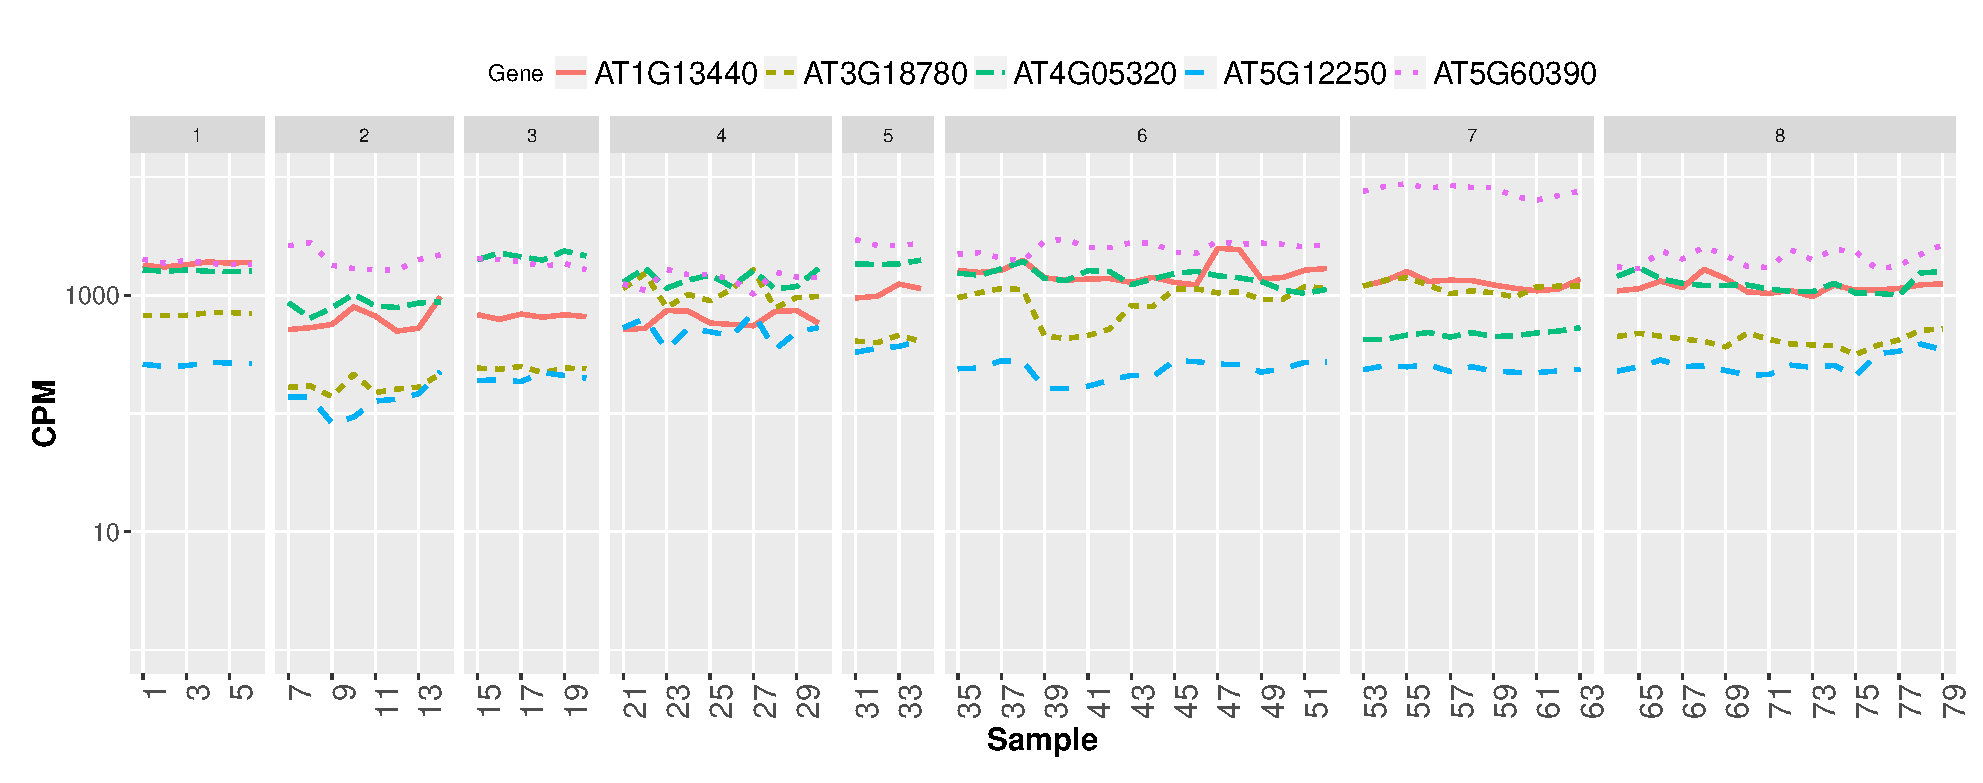
\includegraphics[scale=0.4]{../Figures/A1.eps}
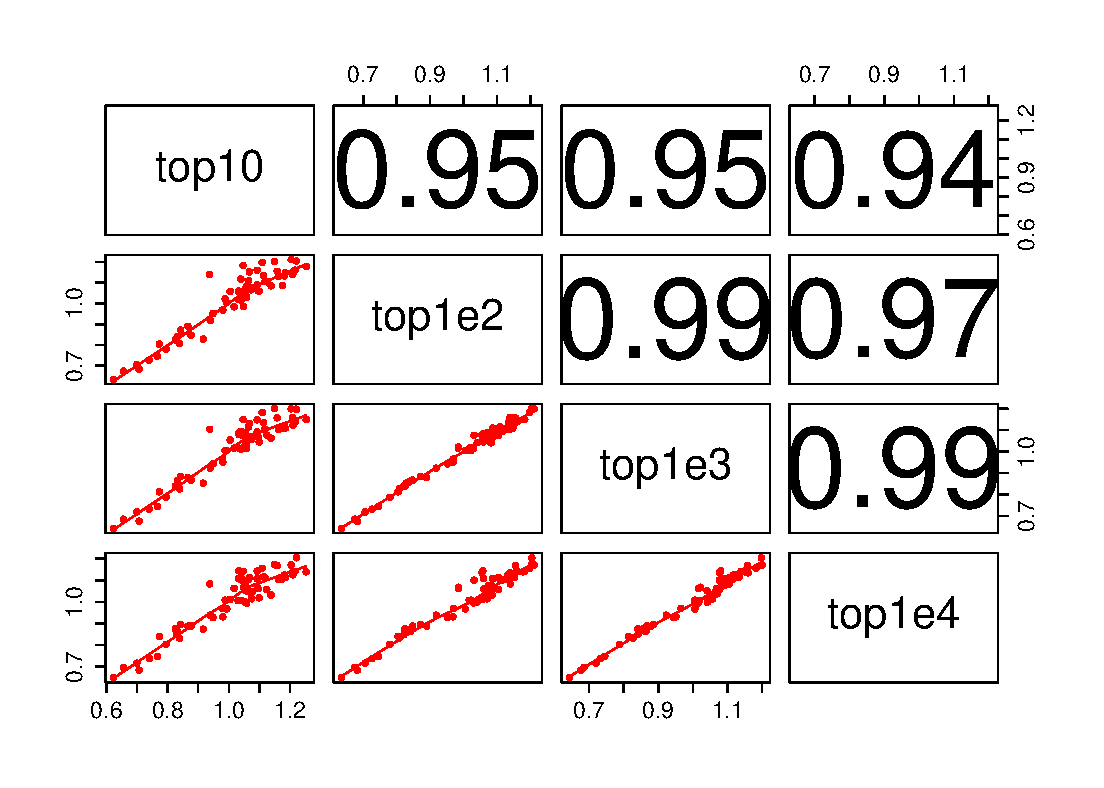
\includegraphics[scale=0.4]{../Figures/B1.eps}
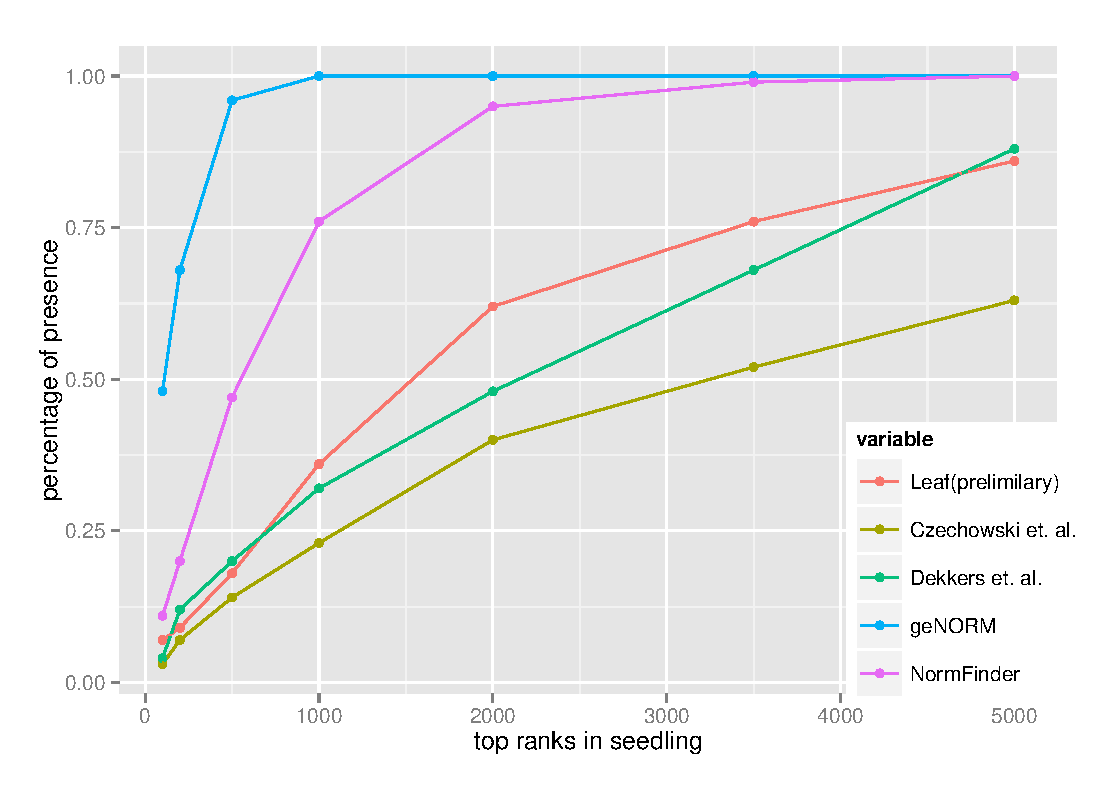
\includegraphics[scale=0.4]{../Figures/C1.eps}

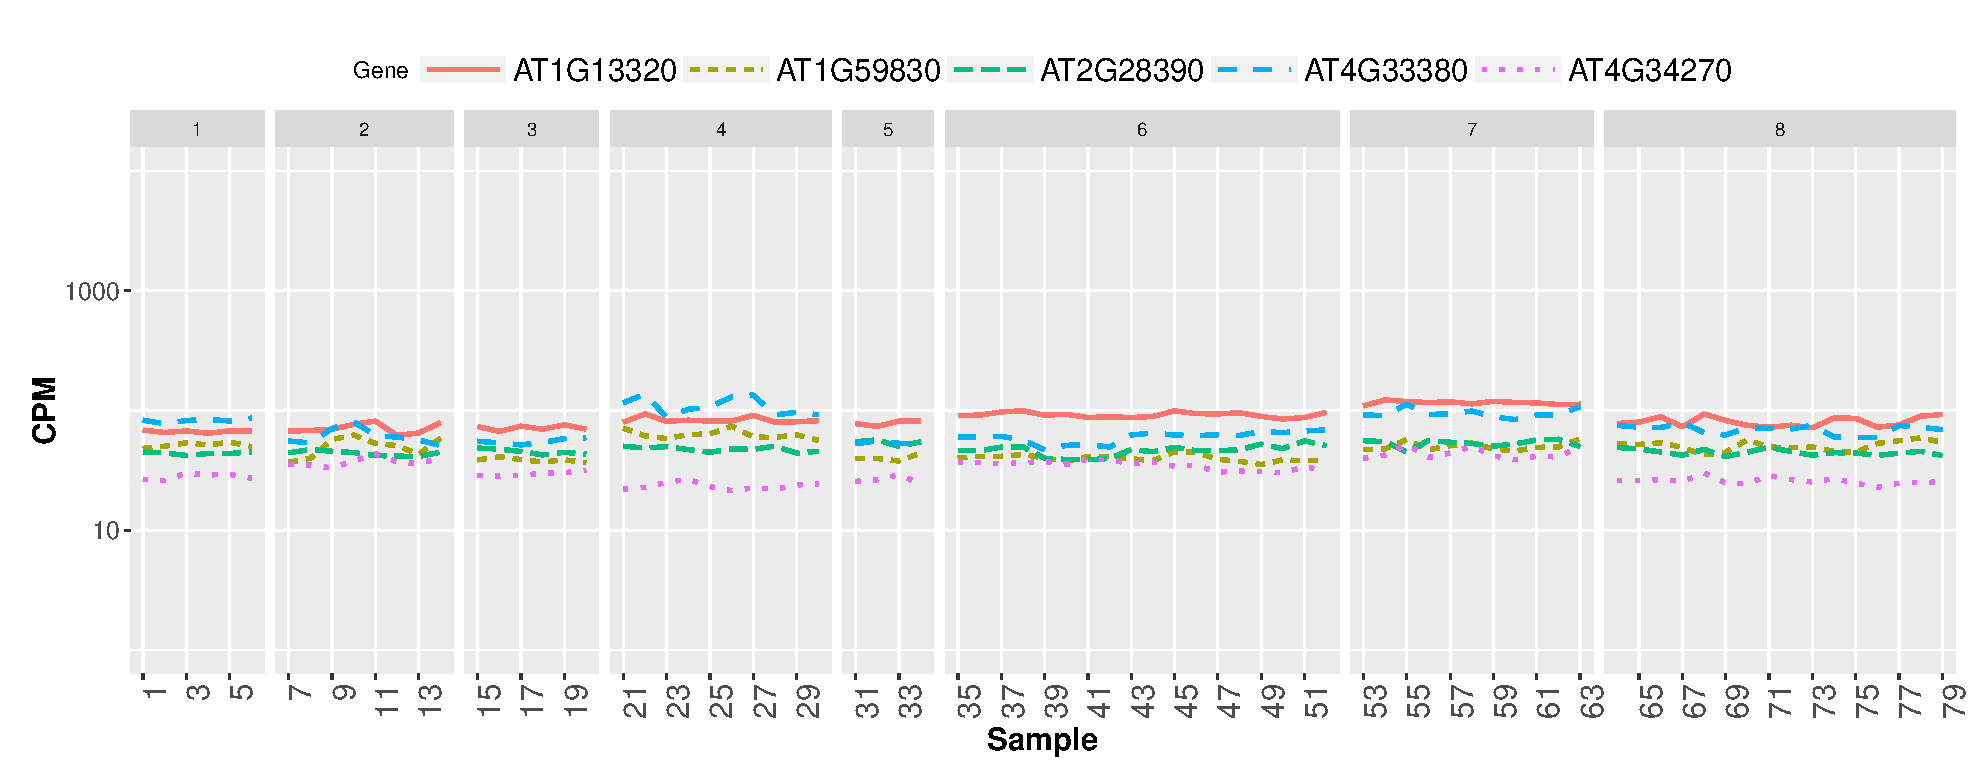
\includegraphics[scale=0.4]{../Figures/A2.eps}
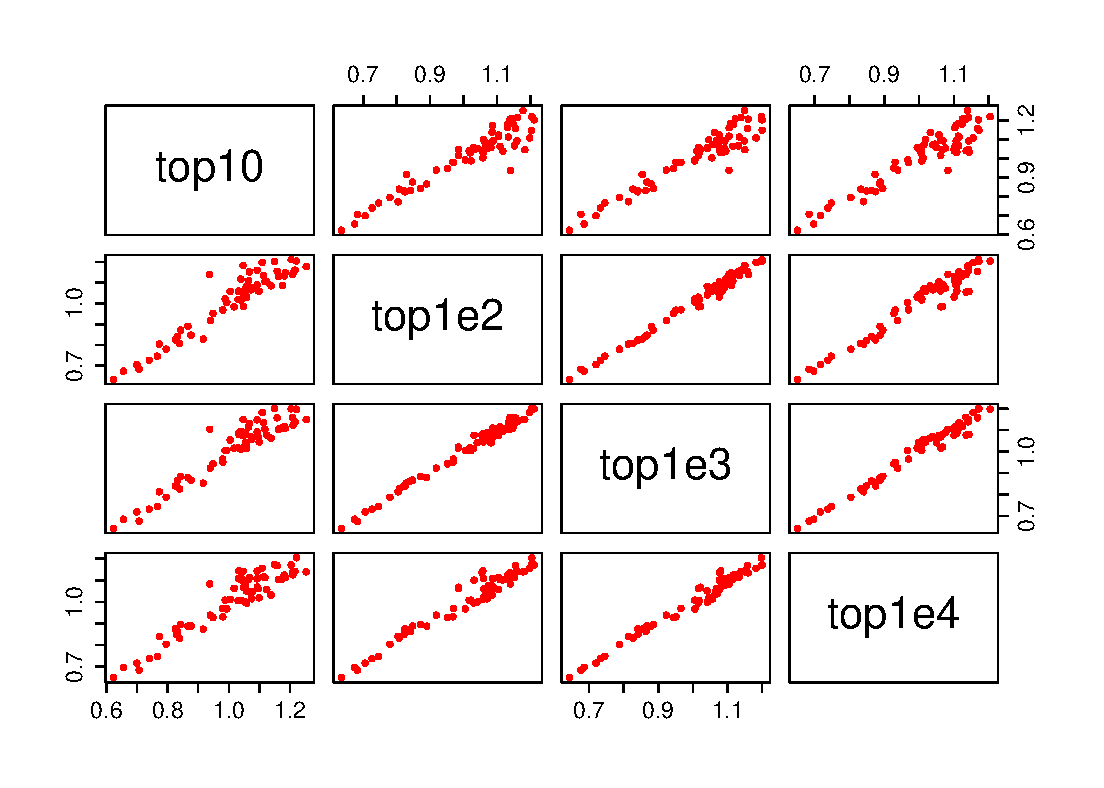
\includegraphics[scale=0.4]{../Figures/B2.eps}
\includegraphics[scale=0.4]{../Figures/C2.eps}

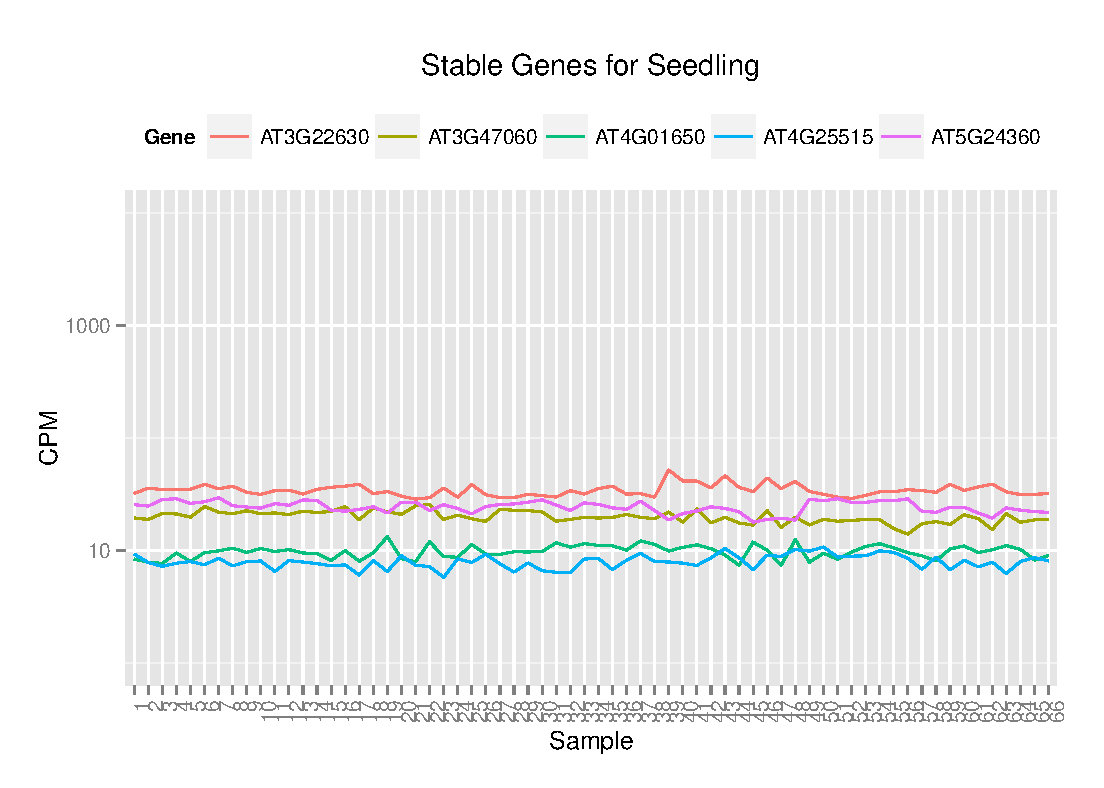
\includegraphics[scale=0.4]{../Figures/A3.eps}
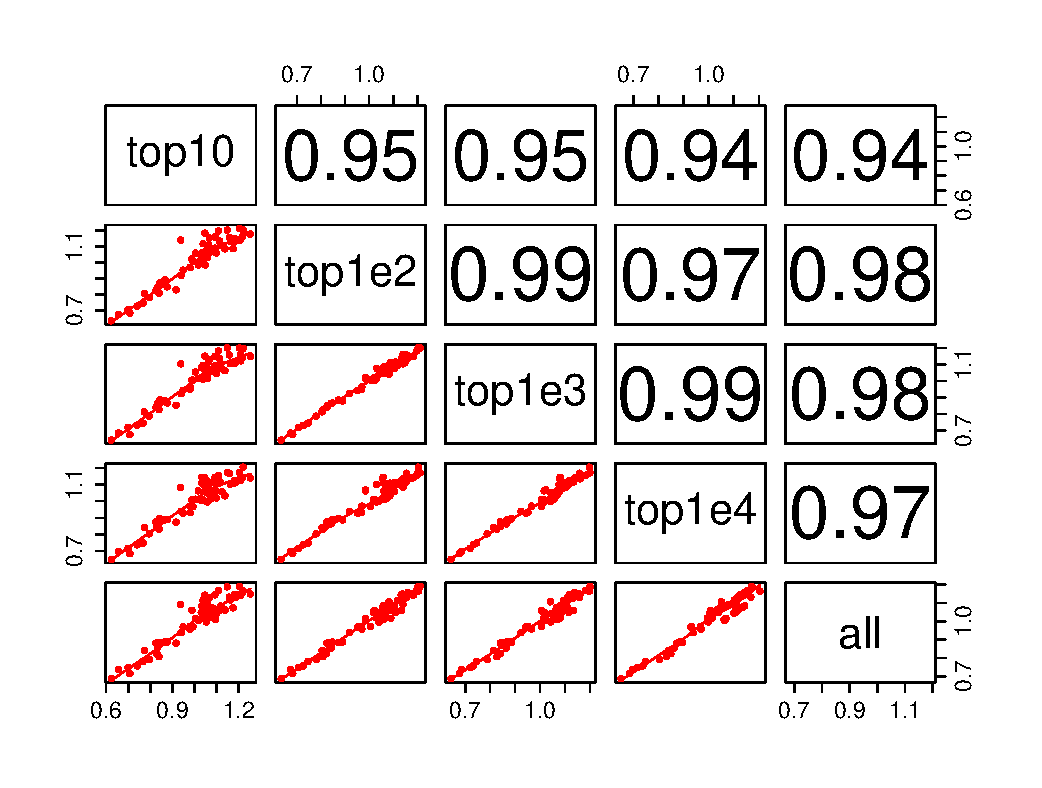
\includegraphics[scale=0.4]{../Figures/B3.eps}
\includegraphics[scale=0.4]{../Figures/C3.eps}
\caption{{\small{\label{fig:scaled_diss} RNA-Seq expression levels of traditional reference genes in set 1(A), set 2 (D) and set 3 (G)}; expression levels of 5 stably expressed genes by \cite{czechowski2005genome}, RNA-Seq data set 1 (B), set 2 (E), and set 3 (H); expression levels of top 5 stably expressed genes identified by GLMM, RNA-Seq data set 1 (C), set 2 (F), and set 3 (I) }}
\end{center}
\end{figure} 
\end{landscape}
Figure 3 shows the relative ranks of top 100 stable gene (developmental series) listed in Czechowski paper, and 50 stable genes (Arabidopsis thaliana seed) listed in \cite{dekkers2012identification}. Of the 91 genes that appears in the gene lists we analyzed, about 30\% are in our top 1000 list (29 for Set 1, 31 for Set 2 and 27 for Set 3, respectively), about 85\% in top 5000 list. On the contrast, the list provided by Dekkers are less stable, possibly because transcriptomes of seed are a bit different from other tissues.

 \begin{figure}[h!]
\begin{center}
\includegraphics[scale=0.4]{../Figures/crez1.eps}
\includegraphics[scale=0.4]{../Figures/dekker1.eps}
\includegraphics[scale=0.4]{../Figures/crez2.eps}
\includegraphics[scale=0.4]{../Figures/dekker2.eps}
\includegraphics[scale=0.4]{../Figures/crez3.eps}
\includegraphics[scale=0.4]{../Figures/dekker3.eps}
\caption{\label{fig:scaled_diss} rank of top 100 stably expressed genes identified by Czechowski in Set 1 (A), Set 2 (B), Set 3 (C); rank of top 50 stably expressed genes identified by Dekkers in Set 1(D), Set 2 (E), Set 3 (F).  }
\end{center}
\end{figure}

Another observation is that stably expressed genes are more consistent within RNA-Seq data than between RNA-Seq and microarray data.  Supplementary figures present rank-rank plot of Set 1 versus Set 2 and Set 1 versus Set 3.  The overlaps for top ranked stably expressed genes are significantly larger, as summarized in table below.
\begin{center}
\begin{table}[h]
\begin{tabular}{lrrr}
     & &\multicolumn{2}{c}{Overlap} \\ \cmidrule(r){3-4}
\multirow{4}{*}{Seedling Data} &Top Rank & Tissue Data  & Leaf Data  \\  \hline
              	   &100  & 8 &9  \\
                  &200  & 21 &27 \\
                   &500  &100  &94 \\
                    &1000  &289  &292 \\ \hline
\end{tabular}
\end{table}

\end{center}

\subsection{Normalization}
One particular goal of this work is to find reference genes for normalization. As a justification, we used stably expressed genes to see how normalization factors vary by choosing different lists of reference genes.   In a series of evaluations, we chose top 10, 100, 1000, 10000 stably expressed genes as reference genes, and then calculated normalization factors \citep{anders2010differential}(AH2010) for each sample in Set 1, Set 2 and Set 3. It can be seen from Figure 4 that normalization factors are more consistent when choosing 100, 1000, or 10000 reference genes in all 3 scenarios. 

 \begin{figure}[h!]
\begin{center}
\includegraphics[scale=0.3]{../Figures/norm1_u.eps}
\includegraphics[scale=0.3]{../Figures/norm2_u.eps}
\includegraphics[scale=0.3]{../Figures/norm3_u.eps}

\caption{\label{fig:scaled_diss} matrix plot of normalization factors by choosing top 10, 100, 1000, 10000 stably expressed genes for Set 1 (A), Set 2 (B), and Set 3 (C). }
\end{center}
\end{figure}

{\color{blue} is it necessary to use another different data set to verify the consistency of normalization factors?}

 \begin{figure}[h!]
\begin{center}
\includegraphics[scale=0.3]{../Figures/r3.eps}
\caption{\label{fig:scaled_diss} normalization factors of seedling data with stable genes from tissue }
\end{center}
\end{figure}

  \section{Discussion}

  \subsection{Alternative method}
A widely adopted way of conducting RNA-Seq data analysis begins with the assumption that $Y_{jkl}$ follows a negative binomial distribution (a.k.a Poisson-Gamma mixture). Both the model in this paper and NB regression start by specifying a Poisson distribution on $Y$, i.e. $Y\sim \text{Poi}(\mu)$, the subtlety lies the way how the mean parameter is modeled. Instead of imposing a log-normal distribution on $\mu$ for Poisson regression, under NB distribution $\mu$ has a gamma distribution.  In light of this, we also tried alternative approach-the negative binomial regression- to estimate between experiment and between treatment variation. Specifically,  for each gene, we assume $Y_{jkl}\sim NB(\mu_{jkl}, \phi)$ with the link function
 \[\log(\mu_{jkl})= \xi + \log(R_{jkl}N_{jkl}) + \alpha_l + \beta_{k(l)}\]
where similarly, $\alpha_l$ is the random effect for experiment, and $\beta_{k(l)}$ is random treatment effect nested in experiments.  The only difference is that the dispersion $\phi$, rather than variance of biological sample in Poisson regression, is estimated in NB setting. We saw no significant difference in estimating the variance components between these two approaches. The NB regression is done by \verb"glmer.nb()" in \verb"lme4" package\citep{bates2012lme4} and \verb"glmmadmb()" in \verb"glmmADMB" package\citep{bolker2012getting}. Unfortunately, both implementations of NB regression experienced convergence failure. \\

A limitation of this study is that the inherent design structures are not taken into account unless when the experiment is a case-control (single factor) study. Our concern is two fold: one, although we collected more than 150 samples, they are far from enough for a complicated design structure because usually there are only 2 or 3 replicates within each treatment;  two, no available package allows for such designs under generalized linear mixed model.  In practice, if there is more than 1 factors in the experiment, we just treat it as single-factor and multiple-level. 

\subsection{Normalization}
 Among them,  The trimmed mean of M-values in edgeR and DESeq normalization in DESeq  (do I need to cite their paper? Not DE = stable?) are based on the hypothesis that most genes are not DE. 
\subsection{Biological interpretation???}
% \subsection{About the result}
%  We compared our results with earlier literature, and found our list of stably expressed genes are significantly diffenrent from previous works in microarray experiments. For the top 200 SEGs we identified from different tissues of arabidopsis, only 5 are present in Czechowski paper(2005) where they listed 100 SEGs under various conditions, and 3 are presented in Dekkers (2012) where a list of 50 SEGs were obtained by analysis of arabidopsis seed data. It is worth noting that these two sets of genes have only 3 in common. \\
%  
%  The discrepency may be due to the difference between microarray and RNA-Seq technologies.  Technical issues inherent to microarray probe performance, such as cross-hybridization and limited detection range of individual probes might contribute to contamination of data quality.  Alternative explanation of such discrepency might be limited source of RNA-Seq data, which prevented us from doing a more exhaustive research. 
%  

\section{Supplementary Material}
The details of experimental data is summarized as below

\subsection{Set 1}
\begin{landscape}
\begin{table}
\footnotesize
\centering
\begin{tabular}{p{2cm}p{2cm}p{1cm}p{4cm}p{2.4cm}p{3cm}p{4cm}} \hline
GEO Number &Tissue cluster & sample Size & Description & Age  &Col Name & Platform\\ \hline
GSE37159 &seedling &8	& Col-0, bzr1-1D, pifq and pifq;bzr1-1D  grown on BRZ-containing medium in the dark & 5 days &GSM912634-GSM912641 & Illumina HiSeq 2000\\  \hdashline
GSE38879 &seedling &12 & Transgenic line rve8-1 RVE8::RVE8:GR and rve8-1 treated with DEX or mock with three biological replicates each, 12 samples in total & 7 days  &GSM951349-GSM951360  &Illumina HiSeq 2000\\ \hdashline
GSE43865 &seedling & 6  & wild-type and link1link2 mutant plants were grown for two weeks under continuous white light conditions at 22 degrees centigrades & 9 days & GSM1072464-GSM1072469 &Illumina Genome Analyzer IIx  \\	\hdashline
GSE48767 &seedling & 6 &The wild-type seedlings and the phyA-1 mutant were grown, within each 3 biological replicates available & 4 days   &GSM1184353-GSM1184358, GSM1401633-GSM1401638 &Illumina HiSeq 2000 \\ \hdashline
GSE51119 &seedling  & 10  & homozygous ibh1(SALK 049177), ibl1(SALK 119457), 35Spro:IBH1-GFP and 35Spro:IBL1-GFP were compared to wild type (Col) &10 days  & GSM1239079-GSM1239088 &Illumina HiSeq 2000 \\ \hdashline
GSE51772 &seedling  & 8  & Col-0 and iaa3 were grown on medium for 5 days and treated with mock or 100 nMBL for 4 hr &5 days  & GSM1252262-GSM1252269 &Illumina HiSeq 2000 \\ \hdashline
GSE53078 &seedling &4 & Compare the transcriptome of HBI1-Ox and wild type & 5 days &   GSM1281703-GSM1281706 &Illumina Genome Analyzer \\ \hdashline
GSE57086 &seedling & 6  & cR-grown WT and hid1, three biological replicates for each group & 5 days &GSM1390693-GSM1390698 &GPL13222 \\ \hdashline
GSE58082 &seedling &6  &GFP-FHY1 fhy1-1 transgenic,  fhy1-1 mutant  were grown under the same light conditions used (D4d+FR3h)& 4 days &GSM1400495-GSM1400500 & GPL13222 \\ \hdashline
\end{tabular} 
\end{table}
\end{landscape}


\begin{landscape}
\subsection{Set 2}
\begin{table}
\footnotesize
\centering
\begin{tabular}{p{2cm}p{3cm}p{1cm}p{4cm}p{2.4cm}p{3cm}p{4cm}} \hline
GEO Number &Tissue cluster & sample Size & Description & Age  &Col Name & Platform\\ \hline
 GSE35288 &flower &6  & 3 biological replicates of Col-0 wild type and 3 biological replicates of the hae-3 hsl2-3 double mutant &  stage 15  &SRR401413-SRR401430 &Illumina HiSeq 2000 \\ \hdashline
GSE35408 &Hypocotyl & 10 &bzr1-1D and WT were grown in media containing 1uM PAC and 0 or 2uM PPZ for 4.5 days in dark, then treated with 10uM GA3 or mock solution for 12 hr & 4.5 days  & GSM867674-GSM867678, GSM951964-GSM951968  & Illumina HiSeq 2000 \\ \hdashline
GSE48235 &rosette leaves & 6  & For each condition (water, S1, and S3) the transcriptome was sequenced for two replicates & 9 days & GSM1072464-GSM1072469  &Illumina Genome Analyzer II \\	\hdashline
GSE53952 &seed   & 9 	& Three lines of Arabidopsis, fae1/CL37/PDAT were generated & 7-12 days & GSM1303953-GSM1303979 &Illumina Genome Analyzer IIx etc.. \\  \hdashline
GSE56326 &carpels (15 developing inflorescences) & 8 &Expression profile comparation of wild type, nga mutant and NGA overex- pression &stage 8-13&  & 	Illumina HiSeq 2000 \\ \hdashline
\end{tabular} 
\end{table}
\end{landscape}
\begin{landscape}
\subsection{Set 3}
\begin{table}
\footnotesize
\centering
\begin{tabular}{p{2cm}p{3cm}p{1cm}p{4cm}p{2.4cm}p{3cm}p{4cm}} \hline
GEO Number &Tissue cluster & sample Size & Description & Age  &Col Name & Platform\\ \hline
GSE36626 &leaves & 4 &Analysis of 2 different histone H3 variants and transcriptome in 2 conditions.  & 4 weeks &GSM897684-GSM897687 & Illumina Genome Analyzer IIx \\ \hdashline
GSE39463 &leaves  &12		&Columbia-0 pen2-1 pad4-1 sag101-2 mutant, and samples were collected at 24 hours post inoculation (hpi) of Bgh & & &Illumina HiSeq 2000 \\ \hdashline
GSE48235 &leaves & 6  & For each condition (water, S1, and S3) the transcriptome was sequenced for two replicates & 9 days & GSM1072464-GSM1072469  &Illumina Genome Analyzer II \\	\hdashline
GSE51304 &leaves  & 18 &Bisulfite-seq data for cmt2-7 single mutants, cmt3 single mutants, drm1/2 double mutants, drm1/2 cmt3 triple mutants are collected  & 3 weeks & GSM1242374-GSM1242391 &GPL13222 \\ \hdashline
GSE54677 & leaves   &20  &Col morc1 morc2 morc6 and their double mutants. For each sample, two biological replicates were performed &adult & GSM1321694-GSM1321713	 &	GPL13222\\ \hdashline
\end{tabular} 
\end{table}
\end{landscape}


 \begin{figure}[h!]
\begin{center}
\includegraphics[scale=0.5]{../Figures/rank_sl.eps}
\includegraphics[scale=0.5]{../Figures/rank_st.eps}
\caption{\label{fig:scaled_diss} Rank plot of stably expressed genes,  Set 1 versus Set 2 and Set 3.}
\end{center}
\end{figure}

\newpage


\bibliographystyle{apalike}
\bibliography{mybib}

\end{document}

